\documentclass[10pt,twocolumn]{article}

\usepackage[T5,T1]{fontenc}
\usepackage[utf8]{inputenc}
\usepackage{lmodern}
\usepackage{microtype}
\usepackage[margin=0.72in,columnsep=0.25in]{geometry}
\usepackage{amsmath,amssymb}
\usepackage{booktabs}
\usepackage{array}
\usepackage{tikz}
\usepackage{listings}
\usepackage[unicode]{hyperref}

% Author configuration updated automatically by dist/set-author.py
\newcommand{\GapAuthorFullName}{Mike (GAP Project Lead)}
\newcommand{\GapAuthorAffiliation}{Graph Agent Protocol Contributors}
\newcommand{\GapAuthorEmail}{contributors@gap-protocol.local}
\newcommand{\GapAuthorOrcid}{ORCID pending registration (run dist/set-author.py --orcid ...)}
\newcommand{\GapRepoUrl}{https://github.com/mike/GraphProtocol}


\hypersetup{
  colorlinks=true,
  linkcolor=blue!60!black,
  citecolor=teal!60!black,
  urlcolor=blue!65!black,
  pdftitle={Graph Agent Protocol (GAP)},
  pdfauthor={Duy Duc Nguyen (Infinite Agent Labs)}
}

\lstset{
  basicstyle=\ttfamily\scriptsize,
  breaklines=true,
  frame=single,
  rulecolor=\color{black!25},
  columns=flexible
}

\title{\Large\bfseries Graph Agent Protocol (GAP): Unifying Typed Discovery, Batched Federation, and Zero-Trust Governance for AI Agents}

\author{
  {\fontencoding{T5}\selectfont \GapAuthorFullName} \\
  \small \GapAuthorAffiliation \\
  \small \texttt{\GapAuthorEmail} \quad $\cdot$ \quad {\scriptsize \href{\GapAuthorOrcid}{\texttt{\GapAuthorOrcid}}} \\
  \small Repository: \href{\GapRepoUrl}{\texttt{\GapRepoUrl}}
}

\date{November 16, 2026 \quad (Reference Release \texttt{v0.1.0-rc.1})}

\begin{document}
\maketitle

\begin{abstract}
AI agents increasingly interact with heterogeneous capabilities—REST/OpenAPI services, relational SQL databases, GraphQL subgraphs, gRPC endpoints, CLI utilities, codebases, external MCP tool servers, peer A2A agents, and interactive AG-UI user interfaces. Current practice splits this plane across flat JSON-RPC tool catalogs (Model Context Protocol, MCP), point-to-point agent task endpoints (Agent2Agent, A2A), and ad-hoc frontend streams, incurring $O(N)$ prompt schema inflation, client-orchestrated $N+1$ waterfalls, unpinned mutable tool descriptions vulnerable to rug-pull attacks, and probabilistic authorization leaks when models mediate hot-path routing.

We introduce \textbf{Graph Agent Protocol (GAP)}, the first unified, strongly typed GraphQL-profile gateway and governance layer built around three strictly separated architectural planes: (1) a \emph{Zero-ML deterministic execution plane} combining Cedar policy enforcement, tenant-isolated query planning, DataLoader-style batched federation, and wait-free per-request immutable snapshot pinning backed by a pure-Rust persistent AVL \texttt{OrdMap}; (2) a \emph{three-level progressive discovery plane} (\texttt{\_\_metaGraph} $\rightarrow$ \texttt{\_\_search} $\rightarrow$ \texttt{\_\_type}) exposing a constant five-tool MCP \texttt{2026-07-28} facade (\textbf{651 tokens} at $N \in [10, 1000]$ tools), A2A v1.0 peer workflows, and AG-UI v1.0 (\texttt{/ag-ui}) human-in-the-loop SSE streaming alongside multi-provider System-1 routers (\texttt{@receptron/laya}, \texttt{Jev}, \texttt{gemini-decision-1}) with automatic deterministic fallback (\texttt{INV-17}); and (3) a \emph{zero-trust control plane} enforcing propose-not-activate ingestion, SHA-256 description-hash pinning against rug pulls, DNS-pinned egress SSRF guards, sandboxed subprocess execution, and BLAKE3 hash-chained audit ledgers over dual-stack HTTP/2 + HTTP/3 (\texttt{QUIC RFC 9114}, \texttt{0-RTT} disabled). Implemented across 32 layered Rust crates with zero \texttt{RUSTSEC} advisories and evaluated via our open \texttt{GAP-Bench} and \texttt{RouteBench} suites, GAP reduces cross-branch token usage at $N=1000$ by \textbf{99.0\%} uncached (\textbf{93.5\%} cached) and cuts code-graph context by \textbf{119.3$\times$--208.7$\times$}, while transparently establishing exact crossover regimes ($N \le 50$ cached) where Direct-MCP retains an advantage. Our 28.1\,MB bit-reproducible binary boots in \textbf{1,055.0\,ms} with \textbf{9.32\,MiB} idle RSS, sustains \textbf{1,063.6 req/s} over TCP (\textbf{11.54\,ms} p95) and \textbf{5,013.1 req/s} over persistent multiplexed QUIC (\textbf{2.36\,ms} p95) with zero errors, and recovers from OS \texttt{SIGKILL} in \textbf{28.86\,ms}.
\end{abstract}

% ----------------------------------------------------------------------
\section{Introduction}
\label{sec:intro}

Production AI agents must discover, authorize, compose, and audit operations across disparate data and software systems. Today, two valuable open standards organize parts of this ecosystem: Anthropic's Model Context Protocol (MCP)~\cite{anthropic2024mcp} standardizes vertical tool-to-client invocation over JSON-RPC, while Google's Agent2Agent (A2A) protocol~\cite{google2025a2a} standardizes horizontal task delegation between opaque agents via Agent Cards and asynchronous task state machines.

However, deploying real-world multi-tenant agentic gateways exposes four structural gaps that neither flat MCP servers nor standalone A2A endpoints resolve together:
\begin{enumerate}
  \item \textbf{Context Explosion and Join Waterfalls.} Direct-MCP serializes flat JSON Schema tool catalogs upfront, growing linearly from 1,904 tokens at $N=10$ tools to \textbf{203,421 tokens} at $N=1000$ (\S\ref{sec:eval}). Even after tool selection, flat RPC invokes cross-backend entities via agent round-trips ($O(M)$ joins in context), wasting latency and reasoning budget.
  \item \textbf{Mutable Metadata and Semantic Rug Pulls.} Recent security analyses demonstrate that unpinned MCP tool descriptors suffer tool poisoning, semantic prompt lures, and post-approval rug pulls~\cite{song2025beyond,wang2025mcptox,arxiv2512_06556}. Unchecked upstream error strings and free-form outputs further smuggle instructions directly back into model context.
  \item \textbf{Conflating Discovery with Execution and Authz.} Research systems that embed neural tool classifiers or LLM routers inside every request path add tens to hundreds of milliseconds per hop, introduce non-deterministic drift into typed queries, and risk bypassing formal authorization guarantees.
  \item \textbf{Lack of Unified Graph Semantics Over Heterogeneous Sources.} Treating APIs, SQL tables, code trees, and peer agents as isolated RPC tools forces the LLM itself to act as query planner, schema joiner, and pagination state manager.
\end{enumerate}

We propose \textbf{Graph Agent Protocol (GAP)}, a unified typed protocol and reference implementation designed around a foundational discipline: \emph{use deterministic typed graphs, compilers, and policy engines wherever structure exists, and confine probabilistic retrieval strictly to bounded, calibrated intent discovery}. Rather than replacing existing ecosystems on day one, GAP compiles an RFC-2119 typed GraphQL profile (\textbf{GAP-QL}) behind both native GraphQL-over-HTTP endpoints and backwards-compatible MCP \texttt{2026-07-28} and A2A v1.0 facades.

\paragraph{Contributions.} This paper makes five concrete, reproducible contributions:
\begin{itemize}
  \item \textbf{Three-Plane Typed Agent Gateway Architecture (\S\ref{sec:arch}--\S\ref{sec:proto}):} Formal separation of deterministic hot execution, three-level progressive discovery (\texttt{L0/L1/L2}), and zero-trust snapshot control governed by 20 testable architectural invariants (\texttt{INV-01}--\texttt{INV-20}).
  \item \textbf{Zero-Trust Governance Controls (\S\ref{sec:sec}):} Combine Cedar default-deny policies~\cite{cutler2024cedar}, tenant-keyed isolation across caches/stores/audits, description-hash pinning with fail-closed \texttt{DRIFT} freeze against MCP rug pulls, DNS-pinned SSRF egress defense, OS sandboxing, and tamper-evident BLAKE3 audit chains.
  \item \textbf{Empirical Router \& Conformal Gating Discovery (\S\ref{sec:eval}):} Using \texttt{RouteBench}, we prove why default zero-shot neural System-1 checkpoints fail deployment gates (\textbf{14.29\%} debiased top-1 at 73.85\,ms p95), validating our fail-safe architectural choice to ship deterministic BM25+structural routing (\textbf{95.24\%} test / \textbf{97.22\%} held-out top-1 at \textbf{0.887\,ms} p95) without breaking protocol semantics.
  \item \textbf{Honest Crossover Benchmarks (\texttt{GAP-Bench}) \& Negative Results:} We measure Direct-MCP vs.\ GAP across uncached and 0.10$\times$ prefix-cached regimes for $N \in \{10, 50, 200, 1000\}$ and quantify both massive gains (up to \textbf{95.34$\times$} on joins, \textbf{208.68$\times$} on code graphs) and exact negative crossover cells ($N \le 50$ cached flat RPC; X-1 wire columnarization deferral).
  \item \textbf{Full Rust Reference System \& Verifiable Artifacts (\S\ref{sec:impl}):} 32 layered crates, 6 reference connectors, three-axis inbound/outbound protocol facades (MCP, A2A, AG-UI), 136 verified conformance tests, bit-reproducible release artifacts, and single-command local verification scripts.
\end{itemize}

% ----------------------------------------------------------------------
\section{System Model, Threat Model, and Invariants}
\label{sec:arch}

\begin{figure*}[t]
  \centering
  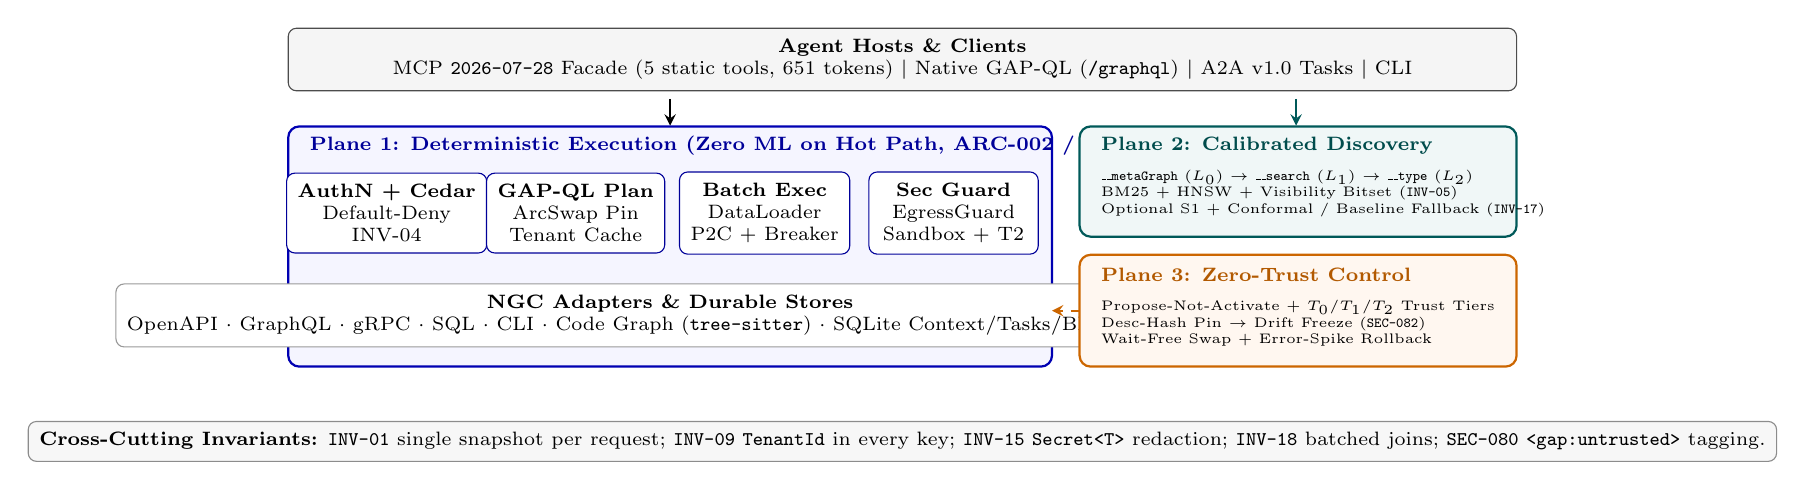
\begin{tikzpicture}[
  box/.style={draw, rounded corners=3pt, align=center, font=\scriptsize, inner sep=4pt, fill=white},
  plane/.style={draw, rounded corners=4pt, thick, inner sep=6pt},
  >=stealth
]
  \node[box, fill=gray!8, minimum width=15.6cm, draw=black!70] (hosts) at (0, 3.6)
    {\textbf{Agent Hosts \& Clients}\\
     MCP \texttt{2026-07-28} Facade (5 static tools, 651 tokens) $\mid$ Native GAP-QL (\texttt{/graphql}) $\mid$ A2A v1.0 Tasks $\mid$ CLI};

  \draw[fill=blue!4, draw=blue!70!black, rounded corners=4pt, thick] (-7.8, -0.3) rectangle (1.9, 2.75);
  \node[anchor=west, font=\scriptsize\bfseries, text=blue!60!black] at (-7.65, 2.50)
    {Plane 1: Deterministic Execution (Zero ML on Hot Path, ARC-002 / INV-01 / INV-02)};

  \node[box, draw=blue!60!black, minimum width=2.15cm, minimum height=0.95cm] (auth) at (-6.55, 1.65)
    {\textbf{AuthN + Cedar}\\Default-Deny\\INV-04};
  \node[box, draw=blue!60!black, minimum width=2.15cm, minimum height=0.95cm] (plan) at (-4.15, 1.65)
    {\textbf{GAP-QL Plan}\\ArcSwap Pin\\Tenant Cache};
  \node[box, draw=blue!60!black, minimum width=2.15cm, minimum height=0.95cm] (exec) at (-1.75, 1.65)
    {\textbf{Batch Exec}\\DataLoader\\P2C + Breaker};
  \node[box, draw=blue!60!black, minimum width=2.15cm, minimum height=0.95cm] (guard) at (0.65, 1.65)
    {\textbf{Sec Guard}\\EgressGuard\\Sandbox + T2};

  \node[box, draw=black!40, minimum width=9.2cm, minimum height=0.8cm] (ngc) at (-2.95, 0.35)
    {\textbf{NGC Adapters \& Durable Stores}\\
     OpenAPI $\cdot$ GraphQL $\cdot$ gRPC $\cdot$ SQL $\cdot$ CLI $\cdot$ Code Graph (\texttt{tree-sitter}) $\cdot$ SQLite Context/Tasks/BLAKE3 Audit};

  \draw[fill=teal!6, draw=teal!70!black, rounded corners=4pt, thick] (2.25, 1.35) rectangle (7.8, 2.75);
  \node[anchor=west, font=\scriptsize\bfseries, text=teal!60!black] at (2.4, 2.50) {Plane 2: Calibrated Discovery};
  \node[anchor=west, font=\tiny, align=left] at (2.4, 1.90)
    {\texttt{\_\_metaGraph} ($L_0$) $\rightarrow$ \texttt{\_\_search} ($L_1$) $\rightarrow$ \texttt{\_\_type} ($L_2$)\\
     BM25 + HNSW + Visibility Bitset (\texttt{INV-05})\\
     Optional S1 + Conformal / Baseline Fallback (\texttt{INV-17})};

  \draw[fill=orange!6, draw=orange!80!black, rounded corners=4pt, thick] (2.25, -0.3) rectangle (7.8, 1.12);
  \node[anchor=west, font=\scriptsize\bfseries, text=orange!70!black] at (2.4, 0.87) {Plane 3: Zero-Trust Control};
  \node[anchor=west, font=\tiny, align=left] at (2.4, 0.25)
    {Propose-Not-Activate + $T_0/T_1/T_2$ Trust Tiers\\
     Desc-Hash Pin $\rightarrow$ Drift Freeze (\texttt{SEC-082})\\
     Wait-Free Swap + Error-Spike Rollback};

  \node[box, fill=gray!6, draw=black!45, minimum width=15.6cm, align=left] (inv) at (0, -1.25)
    {\textbf{Cross-Cutting Invariants:} \texttt{INV-01} single snapshot per request; \texttt{INV-09} \texttt{TenantId} in every key; \texttt{INV-15} \texttt{Secret<T>} redaction; \texttt{INV-18} batched joins; \texttt{SEC-080} \texttt{<gap:untrusted>} tagging.};

  \draw[->, thick] (-2.95, 3.10) -- (-2.95, 2.76);
  \draw[->, thick, draw=teal!70!black] (5.0, 3.10) -- (5.0, 2.76);
  \draw[->, dashed, thick, draw=orange!80!black] (2.25, 0.41) -- (1.90, 0.41);
\end{tikzpicture}


  \caption{Three-plane architecture of GAP. Plane 1 executes typed queries and authorization with zero ML models and wait-free per-request snapshot pinning (\texttt{INV-01}, \texttt{INV-02}). Plane 2 provides three-level schema discovery with deterministic fallback (\texttt{INV-17}). Plane 3 governs ingestion proposals, rug-pull drift pinning (\texttt{SEC-082}), and wait-free RCU snapshot publication.}
  \label{fig:arch}
\end{figure*}

Figure~\ref{fig:arch} illustrates the complete topology separating untrusted external branches, calibrated intent discovery, and deterministic execution.

\subsection{Trust Tiers and Threat Matrix}
Every downstream backend (\emph{branch}) belongs to one of three explicit trust tiers:
\begin{itemize}
  \item \textbf{$T_0$ (Signed Internal Platform):} Verified Ed25519 \texttt{branch.manifest.json} signatures rooted in configured organization public keys; signature mismatch immediately downgrades the branch to $T_2$.
  \item \textbf{$T_1$ (Admin-Approved):} Operator-reviewed branches pinned by cryptographic schema (\texttt{spec\_hash}) and operation description hashes (\texttt{desc\_hash}).
  \item \textbf{$T_2$ (Untrusted / External / Discovered):} Default tier for newly encountered sources. Outputs are scrubbed, length-capped, and wrapped deterministically inside \texttt{<gap:untrusted source="...">...</gap:untrusted>} envelopes whose internal closing tags are HTML-escaped so upstream text cannot hijack downstream agent prompts. Executable processes at $T_2$ are refused fail-closed without OS sandbox availability.
\end{itemize}

Our threat model enumerates 17 protocol-level attack vectors (\texttt{spec/07-security.md} \S15): cross-tenant plan cache collisions, prompt injection via branch descriptions/results/errors, post-approval tool rug pulls, tool shadowing across identically named connectors, irreversible mutation induction via spoofed MCP hints (\texttt{readOnlyHint}), DNS-rebinding/octal/IPv6-mapped SSRF against cloud metadata (\texttt{169.254.169.254}), path-traversal in local CLI/code connectors, bearer-token forwarding leaks, log/error canary leakage, $O(N)$ GraphQL DoS queries, peer-delegation cycles, and audit-log tampering.

\subsection{Core Architectural Invariants}
To prevent architectural erosion across contributors and AI coding agents, GAP binds every runtime module to 20 explicit invariants (\texttt{INV-01}--\texttt{INV-20}), continuously audited in CI by static layering checks (\texttt{tools/check\_layers.py}) and traceability rules (\texttt{tools/spec\_trace.py --strict}). Key invariants include:
\begin{itemize}
  \item \textbf{\texttt{INV-01} / \texttt{INV-02} (Snapshot Pinning \& Lock-Free Hot Path):} Each incoming request reads an atomic \texttt{Arc<Snapshot>} backed by a pure-Rust persistent AVL \texttt{OrdMap} once upon ingress and pins that exact generation until completion; read paths forbid \texttt{Mutex}, \texttt{RwLock}, and \texttt{DashMap}.
  \item \textbf{\texttt{INV-04} (Deterministic Policy Enforcement):} Cedar policies evaluate cleanly before any connector invocation; \texttt{forbid} overrides \texttt{permit}, and \texttt{IRREVERSIBLE} or \texttt{UNKNOWN} mutations fail closed without an explicit distinct-approver authorization context.
  \item \textbf{\texttt{INV-05} (Authorization-Aligned Visibility):} Discovery indexes enforce per-principal visibility bitsets before ranking so forbidden elements neither appear in \texttt{\_\_search} nor distort top-$k$ ordering.
  \item \textbf{\texttt{INV-08} / \texttt{INV-09} (Pinned Descriptions \& Tenant Scoping):} Planners read exclusively sanitized, admin-pinned descriptions; every plan cache key, store row, rate-limit bucket, and audit log is keyed by resolved \texttt{TenantId}.
  \item \textbf{\texttt{INV-17} / \texttt{INV-18} / \texttt{INV-20}:} S1 inference may never gate typed execution and falls back cleanly on timeout/absence; remote cross-branch joins execute in batched $O(\lceil U/B\rceil)$ frames; multi-hop peer tasks propagate decremented hop counters and reject delegation cycles.
\end{itemize}

% ----------------------------------------------------------------------
\section{Protocol Design: GAP-QL, Progressive Disclosure, and Federation}
\label{sec:proto}

\subsection{GAP-QL as a Strict GraphQL Profile}
Earlier exploratory designs extended GraphQL with custom grammar keywords (such as \texttt{traverse} and \texttt{federate}), breaking standard parser ecosystems and invalidating LLM pretraining priors~\cite{hartig2018graphql}. GAP therefore defines \textbf{GAP-QL} strictly as a \emph{valid GraphQL profile} parsed by \texttt{apollo-compiler}. Schema capabilities—root queries (\texttt{\_\_metaGraph}, \texttt{\_\_search}, \texttt{\_\_type}), mutations with mandatory side-effect directives (\texttt{@sideEffect(level)}), authorization scopes (\texttt{@requiresScope}), and cross-branch joins (\texttt{@join})—are modeled solely via standard root fields, object types, and directives. Business/domain rejections preserve GraphQL-over-HTTP conventions (HTTP 200 with structured \texttt{errors[]} and stable string codes such as \texttt{GAP\_FORBIDDEN}, \texttt{GAP\_RATE\_LIMITED}, and \texttt{GAP\_ABSTAINED}).

\subsection{Three-Level Progressive Disclosure \& Facade Parity}
Rather than flooding client context with $O(N)$ flat tool schemas, GAP exposes a fixed \textbf{five-tool MCP \texttt{2026-07-28} facade} (\texttt{gap\_search}, \texttt{gap\_describe}, \texttt{gap\_query}, \texttt{gap\_mutate}, \texttt{gap\_task}), holding client \texttt{tools/list} overhead invariant at \textbf{651 tokens} under the \texttt{GQL-022} estimator $\lceil 10 \cdot \text{bytes} / 36 \rceil$:
\begin{enumerate}
  \item \textbf{$L_0$ (\texttt{\_\_metaGraph} / \texttt{gap\_describe}):} Returns registered branch identifiers, operation counts, domain tags, and concise synopses (58 tokens at 2 branches; 2,777 tokens at 100 branches).
  \item \textbf{$L_1$ (\texttt{\_\_search} / \texttt{gap\_search}):} Executes hybrid lexical BM25 + dense vector HNSW retrieval filtered by visibility bitsets (\texttt{INV-05}), returning ranked minimal candidate signatures.
  \item \textbf{$L_2$ (\texttt{\_\_type} / \texttt{gap\_describe(names)}):} Hydrates exact GraphQL field definitions, input types, and \texttt{@sideEffect} annotations exclusively for selected types prior to invoking \texttt{gap\_query} or \texttt{gap\_mutate}.
\end{enumerate}

\subsection{Native Graph Connectors (NGC), Three-Axis Facades, Dual-Stack HTTP/2 + HTTP/3, and Joins}
Each downstream source implements a uniform gRPC/stdio protobuf contract (\texttt{Describe}, \texttt{BatchQuery}, \texttt{Mutate}, \texttt{StreamEvents}, \texttt{Ping}). At L4, \texttt{gap-transport} completes all three axes of the open agent ecosystem—vertical tools (\texttt{/mcp} per MCP \texttt{2026-07-28}), horizontal agent delegation (A2A v1.0), and user-facing event/state/interrupt streaming (\texttt{/ag-ui} per AG-UI v1.0, \texttt{ADR-027}, mapping unapproved \texttt{@sideEffect} mutations cleanly to \texttt{RUN\_FINISHED} interrupts and isolating \texttt{T2} outputs inside escaped \texttt{<gap:untrusted>} tags)—concurrently over \textbf{HTTP/1.1+HTTP/2 TCP} (advertising \texttt{Alt-Svc: h3=":<port>"; ma=86400}) and \textbf{HTTP/3 over QUIC} (RFC 9114, TLS 1.3 ALPN \texttt{h3} via \texttt{quinn} + \texttt{h3} per \texttt{ADR-026}/\texttt{OPS-005}). TLS 1.3 \texttt{0-RTT} early data is explicitly disabled (\texttt{max\_early\_data\_size = 0}) so mutations and tool invocations cannot replay across UDP retries, and \texttt{profile = "prod"} fails closed if \texttt{http3\_listen} lacks explicit certificate and key secrets. For optional neural System-1 discovery, \texttt{gap-s1} unifies local Candle checkpoints, \texttt{@receptron/laya} ONNX HTTP bridges, TypeSafe \texttt{Jev} (\texttt{/v1/systemone}), and Google \texttt{gemini-decision-1} (\texttt{/v1beta/decisions}, zero output tokens, up to 1,000 parallel \texttt{choice}/\texttt{score}/\texttt{noul} evaluations, \texttt{ADR-028}) strictly under \texttt{EgressGuard}, \texttt{Secret<T>} redaction, and \texttt{INV-17} deterministic fallback. Cross-branch relationships declared via \texttt{@join(on: ...)} require explicit \emph{data-driven join verification} during ingestion (computing key sketch containment, right-hand uniqueness, null ratios, and cardinality multipliers—never trusting LLM similarity scores alone) before promotion to \texttt{ACTIVE}. During execution, join keys from parent results are deduplicated canonically (normalizing negative zeros and map order) and dispatched in bounded slices of size $B$, eliminating N+1 upstream round-trips (\texttt{INV-18}). Asynchronous workflows execute via A2A-compatible durable tasks (\texttt{Submitted} $\rightarrow$ \texttt{Working} / \texttt{InputRequired} $\rightarrow$ terminal states) backed by leased worker recovery (\texttt{RUN-091}).

% ----------------------------------------------------------------------
\section{Zero-Trust Governance and Snapshot Control}
\label{sec:sec}

\subsection{Deterministic Policy Enforcement (Cedar)}
Authentication verifies HMAC/JWT tokens or BLAKE3-hashed API keys into immutable principal scopes. Every field and mutation checks compiled Cedar policies~\cite{cutler2024cedar} over \texttt{(principal, action, resource, context)} cleanly before planning finishes. To prevent semantic spoofing, downstream MCP annotation hints such as \texttt{readOnlyHint} are ignored at authorization time; mutations without verified \texttt{@sideEffect(level: SAFE\_IDEMPOTENT | REVERSIBLE)} classification default to \texttt{UNKNOWN} and require explicit multi-party approval contexts.

\subsection{Propose-Not-Activate Ingestion \& Rug-Pull Freeze}
New connectors or schema updates never auto-mutate the live graph. Instead, \texttt{gap-ingest} extracts candidate descriptors inside sandboxed workers, scrubs HTML/hidden Unicode and flags imperative prompt-injection lures via the CISG linter, and stores an administrative \texttt{Proposal}. Once approved, GAP records cryptographic hashes (\texttt{spec\_hash}, \texttt{desc\_hash}) per operation. Background polling by \texttt{DriftMonitor} recomputes sanitized description hashes and classifies diffs into \texttt{Cosmetic}, \texttt{SchemaCompatible}, \texttt{SchemaBreaking}, or \texttt{DescriptionChange}. Any breaking schema modification or unapproved description mutation (rug pull) forces the branch immediately into \texttt{BranchStatus::Drift}, freezes active planners onto the previously verified pinned descriptions (\texttt{INV-08}), and triggers operator alerts.

\subsection{Sandboxing, SSRF Egress Guard, and Cryptographic Audit}
All outbound connector traffic traverses \texttt{EgressGuard}, which resolves DNS once, rejects loopback, RFC 1918/4193, CGNAT, multicast, cloud metadata (\texttt{169.254.169.254}), decimal/octal/hex obfuscated IPs, IPv4-mapped IPv6 forms, and HTTP userinfo, and connects directly to the pinned socket IP without re-resolution across at most three non-downgrading redirects. Local CLI/stdio connectors execute under OS process sandboxes (Linux Bubblewrap/\texttt{nsjail} with dropped capabilities and \texttt{no\_new\_privs}; macOS Seatbelt profiles locally) with explicit binary SHA-256 allowlists checked at every launch. Sensitive credentials use \texttt{Secret<T>} wrappers with pattern redaction (\texttt{INV-15}). Security events append into tenant-scoped and system-scoped SQLite ledgers chained by sequential BLAKE3 hashes and exportable as W3C PROV-O JSON-LD artifacts.

\subsection{Wait-Free Snapshot Publishing \& Error-Spike Rollback}
Compiling a new proposal builds an immutable \texttt{Snapshot} generation (supergraph SDL, routing table, visibility bitsets, compiled Cedar policy set) pre-warmed against top plans, atomically published via \texttt{ArcSwap}. Snapshot destruction is offloaded off the swapper thread (\texttt{docs/00-REVIEW.md} F-01), keeping swap latency in the tens of microseconds while busy reader requests observe zero locks or torn views. A post-promotion \texttt{RollbackWatcher} monitors generation-attributable error ratios against baseline over a 60\,s window ($\ge 200$ samples, $> \max(2\times\text{baseline}, \text{baseline} + 2\text{pp})$), triggering automatic one-shot rollback and quarantine of faulty generations.

% ----------------------------------------------------------------------
\section{Reference Implementation \& Verification Rigor}
\label{sec:impl}

GAP is implemented in \textbf{Rust (Edition 2024, pinned toolchain \texttt{1.98.1})} across \textbf{32 workspace crates} arranged strictly into layers \texttt{L0}--\texttt{L6}:
\begin{itemize}
  \item \textbf{Core \& Durability (\texttt{L0}--\texttt{L1}):} \texttt{gap-core}, \texttt{gap-proto} (pure-Rust \texttt{protox} compilation without external \texttt{protoc} runtime risk), \texttt{gap-store} (SQLite context/tasks/audit/idempotency stores with online \texttt{backup\_to}/\texttt{restore\_from} plus opt-in \texttt{store-surreal} isolation keeping BSL crates completely out of default \texttt{Cargo.lock}), \texttt{gap-index}, \texttt{gap-sec}, \texttt{gap-models}.
  \item \textbf{Protocol, Routing \& Adapters (\texttt{L2}--\texttt{L4}):} \texttt{gap-ql}, \texttt{gap-plan}, \texttt{gap-exec}, \texttt{gap-route}, \texttt{gap-s1} (isolated \texttt{unsafe}-scoped Candle adapter plus \texttt{receptron-laya}, \texttt{jev}, and \texttt{gemini-decision-1} providers), \texttt{gap-balance}, \texttt{gap-snapshot}, \texttt{gap-ingest}, \texttt{gap-ngc-sdk}, plus six shipped adapters (\texttt{OpenAPI}, \texttt{GraphQL}, \texttt{gRPC}, \texttt{SQL}, \texttt{CLI}, \texttt{Code Graph} using \texttt{tree-sitter}) and inbound/outbound \texttt{gap-mcp}, \texttt{gap-a2a}, and \texttt{gap-agui}.
  \item \textbf{Server, Conformance \& CLI (\texttt{L5}--\texttt{L6}):} \texttt{gap-transport} (dual-stack \texttt{HTTP/1.1}+\texttt{HTTP/2} TCP + \texttt{HTTP/3} QUIC via \texttt{quinn} and \texttt{h3}), \texttt{gap-server}, \texttt{gap-conformance}, \texttt{gap-cli} (\texttt{gap} executable supporting 15 operational subcommands including \texttt{serve}, \texttt{doctor}, \texttt{config}, \texttt{models}, \texttt{proposals}, \texttt{snapshot}, \texttt{policy}, \texttt{audit}, \texttt{calibrate}, \texttt{tasks}, and \texttt{purge}).
\end{itemize}

Every non-test crate denies \texttt{unwrap\_used}, \texttt{expect\_used}, \texttt{panic}, \texttt{todo}, and \texttt{unimplemented}, with \texttt{unsafe} code isolated strictly to optional \texttt{gap-s1}. Snapshot trees use an owned zero-\texttt{unsafe} persistent AVL \texttt{OrdMap}, and TLS PEM parsing uses \texttt{rustls-pki-types} directly, yielding zero errors across \texttt{cargo deny check advisories bans licenses sources} (\texttt{ignore = []}). Specification-to-code traceability checks (\texttt{tools/spec\_trace.py --strict}) validate \textbf{362 normative requirements} (\textbf{89 MUST}, \textbf{0 uncovered}) mapped to \textbf{2,515 test markers}. Offline verification passes across:
\begin{itemize}
  \item \textbf{Conformance:} \texttt{133 passed} batch offline conformance tests plus \texttt{2 passed} loopback NGC socket drills (\texttt{135/136}; the sole external differential JS check requires an external \texttt{node}/\texttt{graphql} 16.x directory).
  \item \textbf{Property \& Hardening Suites:} \texttt{365/365} tests passing at \texttt{PROPTEST\_CASES=1024} across 9 crates, 10 fuzz targets with 34 checked-in seed corpora, \texttt{4/4} network-partition/breaker/cancellation chaos tests, \texttt{4/4} soak/rug-pull/quota/two-stage-shutdown tests, and \texttt{3/3} $N-1 \rightarrow N$ SQLite migration + backup/restore drills.
\end{itemize}

% ----------------------------------------------------------------------
\section{Empirical Evaluation}
\label{sec:eval}

We evaluate GAP reproducibly using \texttt{gapbench} (\texttt{bench/results/gapbench/baseline.json}), \texttt{routebench} (\texttt{bench/results/routebench/}), Criterion microbenchmarks (\texttt{m3-baseline.json}), and live process/HTTP drills (\texttt{bench/results/ga\_local/report.json}) on compiled \texttt{--release} builds. All artifacts regenerate offline via single-command harnesses.

\subsection{Discovery Scaling (\texttt{tools/list}, Recall, Latency)}

\begin{figure}[t]
  \centering
  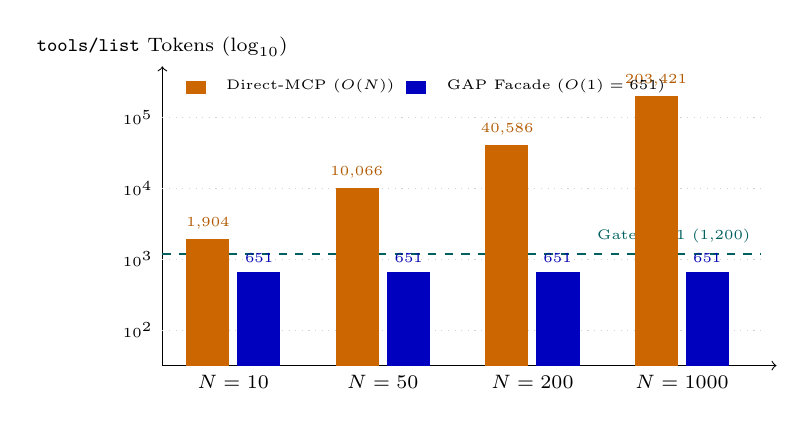
\begin{tikzpicture}[x=1cm, y=1cm]
  \draw[->] (-0.3,0) -- (7.5,0);
  \draw[->] (-0.3,0) -- (-0.3,3.8) node[above, font=\scriptsize] {\texttt{tools/list} Tokens ($\log_{10}$)};
  \draw[dashed, teal!75!black, thick] (-0.3,1.421) -- (7.3,1.421) node[anchor=south east, font=\tiny, text=teal!75!black] {Gate G-F1 (1,200)};
  \draw[gray!35, dotted] (-0.3,0.450) node[left, font=\tiny, text=black] {$10^2$} -- (7.3,0.450);
  \draw[gray!35, dotted] (-0.3,1.350) node[left, font=\tiny, text=black] {$10^3$} -- (7.3,1.350);
  \draw[gray!35, dotted] (-0.3,2.250) node[left, font=\tiny, text=black] {$10^4$} -- (7.3,2.250);
  \draw[gray!35, dotted] (-0.3,3.150) node[left, font=\tiny, text=black] {$10^5$} -- (7.3,3.150);
  \fill[orange!80!black] (0.00,0) rectangle (0.55,1.602);
  \node[above, font=\tiny, text=orange!70!black] at (0.28,1.602) {1,904};
  \fill[blue!75!black] (0.65,0) rectangle (1.20,1.182);
  \node[above, font=\tiny, text=blue!70!black] at (0.93,1.182) {651};
  \node[below, font=\scriptsize] at (0.60,0) {$N=10$};
  \fill[orange!80!black] (1.90,0) rectangle (2.45,2.253);
  \node[above, font=\tiny, text=orange!70!black] at (2.17,2.253) {10,066};
  \fill[blue!75!black] (2.55,0) rectangle (3.10,1.182);
  \node[above, font=\tiny, text=blue!70!black] at (2.83,1.182) {651};
  \node[below, font=\scriptsize] at (2.50,0) {$N=50$};
  \fill[orange!80!black] (3.80,0) rectangle (4.35,2.798);
  \node[above, font=\tiny, text=orange!70!black] at (4.08,2.798) {40,586};
  \fill[blue!75!black] (4.45,0) rectangle (5.00,1.182);
  \node[above, font=\tiny, text=blue!70!black] at (4.72,1.182) {651};
  \node[below, font=\scriptsize] at (4.40,0) {$N=200$};
  \fill[orange!80!black] (5.70,0) rectangle (6.25,3.428);
  \node[above, font=\tiny, text=orange!70!black] at (5.97,3.428) {203,421};
  \fill[blue!75!black] (6.35,0) rectangle (6.90,1.182);
  \node[above, font=\tiny, text=blue!70!black] at (6.62,1.182) {651};
  \node[below, font=\scriptsize] at (6.30,0) {$N=1000$};
  \fill[orange!80!black] (0.0,3.45) rectangle (0.25,3.62) node[right, xshift=4pt, yshift=-2pt, font=\tiny, text=black] {Direct-MCP ($O(N)$)};
  \fill[blue!75!black] (2.8,3.45) rectangle (3.05,3.62) node[right, xshift=4pt, yshift=-2pt, font=\tiny, text=black] {GAP Facade ($O(1) = 651$)};
\end{tikzpicture}

  \caption{MCP \texttt{tools/list} token footprint vs.\ catalog size $N$ (\texttt{GQL-022}). Direct-MCP scales linearly to 203,421 tokens at $N=1000$, while GAP's five-tool facade stays constant at 651 tokens (well below Gate G-F1's 1,200 limit).}
  \label{fig:scaling}
\end{figure}

As shown in Figure~\ref{fig:scaling} and Table~\ref{tab:gapbench}, exporting every downstream tool directly via MCP causes prompt preamble cost to reach 203,421 tokens at $N=1000$ (100 branches). GAP maintains an invariant \textbf{651-token} static schema footprint across all $N$, while its hybrid \texttt{\_\_search} index achieves \textbf{1.0000 Recall@10} across every sweep point at \textbf{0.413\,ms} ($N=10$) to \textbf{3.618\,ms} ($N=1000$) p95—over 10$\times$ faster than the 40\,ms SLO.

\subsection{End-to-End Token Efficiency and Crossover Law}

\begin{figure*}[t]
  \centering
  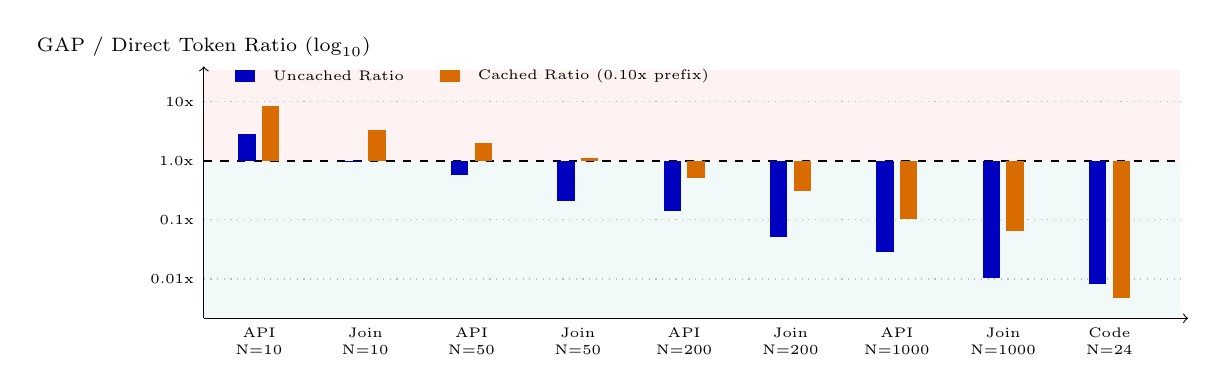
\begin{tikzpicture}[x=1cm, y=1cm]
  \fill[red!5] (0,2.000) rectangle (12.4,3.15);
  \fill[teal!5] (0,0) rectangle (12.4,2.000);
  \draw[->] (0,0) -- (12.5,0);
  \draw[->] (0,0) -- (0,3.2) node[above, font=\scriptsize] {GAP / Direct Token Ratio ($\log_{10}$)};
  \draw[dashed, thick] (0,2.000) node[left, font=\tiny] {1.0x} -- (12.4,2.000);
  \draw[dotted, gray!50] (0,0.500) node[left, font=\tiny, text=black] {0.01x} -- (12.4,0.500);
  \draw[dotted, gray!50] (0,1.250) node[left, font=\tiny, text=black] {0.1x} -- (12.4,1.250);
  \draw[dotted, gray!50] (0,2.750) node[left, font=\tiny, text=black] {10x} -- (12.4,2.750);
  \fill[blue!75!black] (0.44,2.000) rectangle (0.66,2.341);
  \fill[orange!85!black] (0.74,2.000) rectangle (0.96,2.700);
  \node[below, font=\tiny, align=center] at (0.70,0) {API\\N=10};
  \fill[blue!75!black] (1.79,1.986) rectangle (2.01,2.000);
  \fill[orange!85!black] (2.09,2.000) rectangle (2.31,2.394);
  \node[below, font=\tiny, align=center] at (2.05,0) {Join\\N=10};
  \fill[blue!75!black] (3.14,1.819) rectangle (3.36,2.000);
  \fill[orange!85!black] (3.44,2.000) rectangle (3.66,2.223);
  \node[below, font=\tiny, align=center] at (3.40,0) {API\\N=50};
  \fill[blue!75!black] (4.49,1.485) rectangle (4.71,2.000);
  \fill[orange!85!black] (4.79,2.000) rectangle (5.01,2.031);
  \node[below, font=\tiny, align=center] at (4.75,0) {Join\\N=50};
  \fill[blue!75!black] (5.84,1.369) rectangle (6.06,2.000);
  \fill[orange!85!black] (6.14,1.782) rectangle (6.36,2.000);
  \node[below, font=\tiny, align=center] at (6.10,0) {API\\N=200};
  \fill[blue!75!black] (7.19,1.039) rectangle (7.41,2.000);
  \fill[orange!85!black] (7.49,1.621) rectangle (7.71,2.000);
  \node[below, font=\tiny, align=center] at (7.45,0) {Join\\N=200};
  \fill[blue!75!black] (8.54,0.845) rectangle (8.76,2.000);
  \fill[orange!85!black] (8.84,1.261) rectangle (9.06,2.000);
  \node[below, font=\tiny, align=center] at (8.80,0) {API\\N=1000};
  \fill[blue!75!black] (9.89,0.516) rectangle (10.11,2.000);
  \fill[orange!85!black] (10.19,1.109) rectangle (10.41,2.000);
  \node[below, font=\tiny, align=center] at (10.15,0) {Join\\N=1000};
  \fill[blue!75!black] (11.24,0.442) rectangle (11.46,2.000);
  \fill[orange!85!black] (11.54,0.260) rectangle (11.76,2.000);
  \node[below, font=\tiny, align=center] at (11.50,0) {Code\\N=24};
  \fill[blue!75!black] (0.4,3.0) rectangle (0.65,3.15) node[right, xshift=3pt, yshift=-2pt, font=\tiny, text=black] {Uncached Ratio};
  \fill[orange!85!black] (3.0,3.0) rectangle (3.25,3.15) node[right, xshift=3pt, yshift=-2pt, font=\tiny, text=black] {Cached Ratio (0.10x prefix)};
\end{tikzpicture}

  \caption{Token ratio (\texttt{GAP / Direct-MCP}, log scale) across uncached and 0.10$\times$ prompt-cached regimes. Values below $1.0\times$ (green region) indicate GAP savings; values above $1.0\times$ (red region) reveal where small cached catalogs favor Direct-MCP.}
  \label{fig:crossover}
\end{figure*}

\begin{table*}[t]
\centering
\caption{\texttt{GAP-Bench} end-to-end comparison across suites and catalog scales ($N$). Prompt tokens are measured in \texttt{GQL-022} units under uncached and 0.10$\times$ warm-prefix caching models (100\% task success across all cells).}
\label{tab:gapbench}
\scriptsize
\begin{tabular}{@{}lrrrrrrr@{}}
\toprule
Suite & $N$ & Direct Uncached & GAP Uncached & Ratio (U) & Direct Cached & GAP Cached & Ratio (C) \\
\midrule
\texttt{api\_lookup}        & 10   & 2,041.6   & 5,823.0 & 2.852$\times$ & 547.2     & 4,691.9 & 8.575$\times$ \\
\texttt{api\_lookup}        & 50   & 10,205.5  & 5,859.5 & \textbf{0.574$\times$} & 2,385.2   & 4,728.0 & 1.982$\times$ \\
\texttt{api\_lookup}        & 200  & 40,724.3  & 5,865.5 & \textbf{0.144$\times$} & 9,251.2   & 4,734.9 & \textbf{0.512$\times$} \\
\texttt{api\_lookup}        & 1000 & 203,559.5 & 5,878.0 & \textbf{0.029$\times$} & 45,889.1  & 4,747.0 & \textbf{0.103$\times$} \\
\midrule
\texttt{cross\_branch\_join} & 10  & 8,891.8   & 8,517.9 & \textbf{0.958$\times$} & 2,200.5   & 7,383.7 & 3.355$\times$ \\
\texttt{cross\_branch\_join} & 50  & 41,539.8  & 8,547.9 & \textbf{0.206$\times$} & 6,740.7   & 7,413.7 & 1.100$\times$ \\
\texttt{cross\_branch\_join} & 200 & 163,619.8 & 8,547.9 & \textbf{0.052$\times$} & 23,717.4  & 7,413.7 & \textbf{0.313$\times$} \\
\texttt{cross\_branch\_join} & 1000& 814,959.8 & 8,547.9 & \textbf{0.010$\times$} & 114,294.4 & 7,413.7 & \textbf{0.065$\times$} \\
\midrule
\texttt{code\_graph}         & 24  & 141,681.3 & 1,187.4 & \textbf{0.008$\times$} & 137,810.4 & 660.4   & \textbf{0.005$\times$} \\
\bottomrule
\end{tabular}
\end{table*}

Table~\ref{tab:gapbench} and Figure~\ref{fig:crossover} reveal a sharp, predictable \textbf{Crossover Law}:
\begin{enumerate}
  \item \textbf{Where GAP Dominates:} At $N=1000$, GAP slashes uncached \texttt{api\_lookup} tokens by \textbf{97.1\%} (34.6$\times$) and cross-branch join tokens by \textbf{99.0\%} (\textbf{95.34$\times$} uncached, \textbf{15.42$\times$} cached) while halving agent round-trips from 4.0 to 2.0 via batched server-side federation. On codebase comprehension (\texttt{code\_graph}, 24 symbols), typed graph traversal replaces naive multi-file scans (11.0 $\rightarrow$ 1.0 turns), yielding a \textbf{119.32$\times$} uncached and \textbf{208.68$\times$} cached reduction at 100\% accuracy.
  \item \textbf{Where GAP Does Not Win (Negative Cells):} Under small, flat toolsets ($N=10$), Direct-MCP fits all schemas into a single cached prefix turn (547.2 tokens) vs.\ GAP's two-turn discovery workflow (4,691.9 tokens, 8.575$\times$ worse). With 0.10$\times$ prefix caching enabled, parity crosses between $N=50$ and $N=200$ for single lookups and just above $N=50$ for cross-branch joins. Furthermore, our conditional \texttt{@format(as: COLUMNAR)} wire extension (\texttt{X-1}) yielded $<20\%$ end-to-end suite reduction because total tokens are dominated by discovery and round-trips rather than repeated JSON keys; we retained the lock-free internal \texttt{ColumnarTable} codec while formally deferring wire syntax.
\end{enumerate}

\subsection{Neural System-1 vs.\ Deterministic Baseline (\texttt{RouteBench})}

\begin{table}[t]
\centering
\caption{\texttt{RouteBench} evaluation ($n_{\text{test}}=48$ including 6 OOD queries; $n_{\text{held}}=72$; 1,000 bootstrap resamples). Default un-finetuned Laya weights fail accuracy/latency gates, validating \texttt{BASELINE\_FALLBACK}.}
\label{tab:routebench}
\scriptsize
\begin{tabular}{@{}lrrrr@{}}
\toprule
Router & Test Top-1 & Held Top-1 & Test $\text{ECE}_{15}$ & p95 (ms) \\
\midrule
\texttt{baseline} (BM25+Struct) & \textbf{0.9524} & \textbf{0.9722} & 0.7304 & \textbf{0.887} \\
\texttt{s1\_forward} (Laya f32)   & 0.0714 & 0.0278 & 0.0445 & 42.339 \\
\texttt{s1\_debiased} (Laya+PMI)& 0.1429 & 0.0278 & \textbf{0.0303} & 73.851 \\
\bottomrule
\end{tabular}
\end{table}

Table~\ref{tab:routebench} demonstrates why separating ML discovery from core protocol guarantees is essential. Un-finetuned \texttt{laya-candle:f32} weights calibrate well under PMI debiasing ($\text{ECE}_{15}=0.0303 \le 0.05$) yet score only \textbf{14.29\%} top-1 accuracy at 73.85\,ms p95, whereas GAP's deterministic lexical/structural baseline hits \textbf{95.24\%} test top-1 (\textbf{97.22\%} held-out) in \textbf{0.887\,ms}. Under gate \texttt{G-S1}, GAP ships safely in \texttt{BASELINE\_FALLBACK} mode while exposing calibration CLI tooling for domain-finetuned S1 deployment.

\subsection{Runtime Microbenchmarks \& Live Server Crash Drills}

\begin{figure}[t]
  \centering
  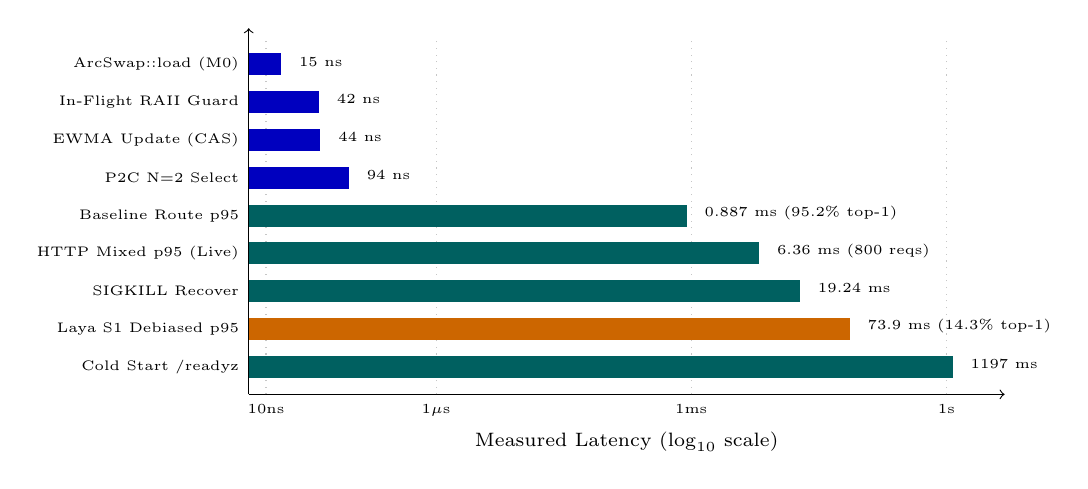
\begin{tikzpicture}[x=1cm, y=1cm]
  \draw[->] (0,0) -- (0,4.65);
  \draw[->] (0,0) -- (9.6,0) node[below, pos=0.5, yshift=-10pt, font=\scriptsize] {Measured Latency ($\log_{10}$ scale)};
  \draw[dotted, gray!45] (0.22,0) node[below, font=\tiny, text=black] {10ns} -- (0.22,4.55);
  \draw[dotted, gray!45] (2.38,0) node[below, font=\tiny, text=black] {$1\mu\mathrm{s}$} -- (2.38,4.55);
  \draw[dotted, gray!45] (5.62,0) node[below, font=\tiny, text=black] {1ms} -- (5.62,4.55);
  \draw[dotted, gray!45] (8.86,0) node[below, font=\tiny, text=black] {1s} -- (8.86,4.55);
  \node[anchor=east, font=\tiny] at (0,4.19) {ArcSwap::load (M0)};
  \fill[blue!75!black] (0,4.05) rectangle (0.41,4.33) node[right, xshift=3pt, yshift=-3pt, font=\tiny, text=black] {15 ns};
  \node[anchor=east, font=\tiny] at (0,3.71) {In-Flight RAII Guard};
  \fill[blue!75!black] (0,3.57) rectangle (0.89,3.85) node[right, xshift=3pt, yshift=-3pt, font=\tiny, text=black] {42 ns};
  \node[anchor=east, font=\tiny] at (0,3.23) {EWMA Update (CAS)};
  \fill[blue!75!black] (0,3.09) rectangle (0.91,3.37) node[right, xshift=3pt, yshift=-3pt, font=\tiny, text=black] {44 ns};
  \node[anchor=east, font=\tiny] at (0,2.75) {P2C N=2 Select};
  \fill[blue!75!black] (0,2.61) rectangle (1.27,2.89) node[right, xshift=3pt, yshift=-3pt, font=\tiny, text=black] {94 ns};
  \node[anchor=east, font=\tiny] at (0,2.27) {Baseline Route p95};
  \fill[teal!75!black] (0,2.13) rectangle (5.56,2.41) node[right, xshift=3pt, yshift=-3pt, font=\tiny, text=black] {0.887 ms (95.2\% top-1)};
  \node[anchor=east, font=\tiny] at (0,1.79) {HTTP Mixed p95 (Live)};
  \fill[teal!75!black] (0,1.65) rectangle (6.48,1.93) node[right, xshift=3pt, yshift=-3pt, font=\tiny, text=black] {6.36 ms (800 reqs)};
  \node[anchor=east, font=\tiny] at (0,1.31) {SIGKILL Recover};
  \fill[teal!75!black] (0,1.17) rectangle (7.00,1.45) node[right, xshift=3pt, yshift=-3pt, font=\tiny, text=black] {19.24 ms};
  \node[anchor=east, font=\tiny] at (0,0.83) {Laya S1 Debiased p95};
  \fill[orange!80!black] (0,0.69) rectangle (7.63,0.97) node[right, xshift=3pt, yshift=-3pt, font=\tiny, text=black] {73.9 ms (14.3\% top-1)};
  \node[anchor=east, font=\tiny] at (0,0.35) {Cold Start /readyz};
  \fill[teal!75!black] (0,0.21) rectangle (8.94,0.49) node[right, xshift=3pt, yshift=-3pt, font=\tiny, text=black] {1197 ms};
\end{tikzpicture}

  \caption{Multi-scale latency spectrum across lock-free RCU primitives (\texttt{ns}), deterministic baseline routing (\texttt{0.887\,ms} p95), live multiplexed HTTP/3 QUIC (\texttt{2.364\,ms} p95) and HTTP/2 TCP (\texttt{11.544\,ms} p95) mixed loads, and \texttt{SIGKILL} recovery (\texttt{28.86\,ms}).}
  \label{fig:latency}
\end{figure}

Figure~\ref{fig:latency} summarizes low-level and live end-to-end runtime timings:
\begin{itemize}
  \item \textbf{Lock-Free Hot Path Primitives:} \texttt{ArcSwap::load} runs in \textbf{15\,ns} (256-reader store median \textbf{22.8\,$\mu$s}, p99 59\,$\mu$s); RAII \texttt{in\_flight} guards take \textbf{42\,ns}, CAS EWMA updates \textbf{44\,ns}, and Power-of-Two-Choices $N=2$ selection \textbf{94\,ns} net median.
  \item \textbf{Bit-Reproducible Release, Dual-Stack HTTP/2 + HTTP/3 Load \& Crash Drills:} Clean offline rebuilds of the 28.1\,MB \texttt{gap} binary (\texttt{28,084,064\,B}) produced identical SHA-256 hashes (\texttt{d3220637...ee965d4c2}). Against live REST+MCP subprocesses over TCP (\texttt{gap serve}, with live \texttt{GET /ag-ui/capabilities} and \texttt{POST /ag-ui} SSE verified), cold startup reached HTTP 200 \texttt{/readyz} in \textbf{1,055.03\,ms} ($\le 2,000$\,ms gate) with \textbf{9.32\,MiB} idle RSS (\textbf{16.30\,MiB} post-load, well under 600\,MiB); across 800 mixed HTTP/1.1 requests (8 threads; 60\% single read, 25\% joined read, 10\% MCP discovery, 5\% probes), GAP sustained \textbf{1,063.6 req/s} with \textbf{0 errors} at 6.744\,ms p50 / \textbf{11.544\,ms} p95 / 18.346\,ms p99. Over native HTTP/3 QUIC (8 multiplexed connections, 800 mixed requests, TLS 1.3 ALPN \texttt{h3}, \texttt{0-RTT} disabled, \texttt{Alt-Svc} advertised) against in-process fixtures, GAP sustained \textbf{5,013.1 req/s} with \textbf{0 errors} at 1.626\,ms p50 / \textbf{2.364\,ms} p95 / 2.710\,ms p99. Following immediate OS \texttt{SIGKILL} (\texttt{-9}), gateway restart served verified queries on \texttt{/readyz} in \textbf{28.86\,ms}.
\end{itemize}

% ----------------------------------------------------------------------
\section{Related Work}
\label{sec:related}

\paragraph{Agent Tool \& Agent-to-Agent Protocols.}
Early tool-augmented LLMs such as Gorilla~\cite{patil2023gorilla} and ToolLLM~\cite{qin2023toolllm} showed retriever-assisted API synthesis and multi-step decision trees across thousands of REST endpoints, yet left multi-tenant authorization, schema drift pinning, and server-side joins out of scope. Anthropic's MCP~\cite{anthropic2024mcp} unified client-tool messaging, while Google's A2A~\cite{google2025a2a} standardized cross-agent tasks and security patterns~\cite{arxiv2504_16902}. Concurrently, academic audits~\cite{song2025beyond,wang2025mcptox,arxiv2512_06556} documented descriptor tool poisoning and rug pulls in naive MCP hosts. Industry MCP GraphQL servers~\cite{apollo_mcp_grafbase} validated progressive schema discovery over GraphQL; GAP generalizes that idea across heterogeneous protocols (OpenAPI, gRPC, SQL, CLI, Code, MCP) inside an auditable, zero-trust Rust gateway with formal cross-branch joins and A2A task integration.

\paragraph{GraphQL Semantics, Policy Engines, and Calibration.}
Hartig and P\'erez~\cite{hartig2018graphql} established formal NL-complete evaluation semantics and enumeration bounds for GraphQL, underpinning our bounded cost-unit limits. Cutler et al.~\cite{cutler2024cedar} designed Cedar in Rust with Lean formal models and SMT analyzability, which GAP adopts for deterministic hot-path enforcement (\texttt{INV-04}). Finally, conformal uncertainty guarantees~\cite{angelopoulos2021conformal} inspire our split-conformal abstention layer and strict \texttt{G-S1} empirical gating in \texttt{RouteBench}.

% ----------------------------------------------------------------------
\section{Limitations and Conclusion}
\label{sec:conclusion}

Several external validation exercises remain gated on multi-day connected cloud infrastructure rather than offline hardware: 72-hour continuous release soak execution, 24-hour nightly libFuzzer campaigns, live frontier LLM API sweeps under \texttt{gapbench}, multi-node 10k\,rps reference runs, and Linux CI OIDC signing/attestation. Likewise, macOS Seatbelt sandboxing serves solely local development while production Linux targets Bubblewrap/Landlock isolation, and locally our HTTP/2 (short-lived Python \texttt{urllib} clients to external subprocesses) and HTTP/3 (persistent multiplexed QUIC connections to in-process fixtures) drills measure distinct transport topologies reported transparently above.

Nevertheless, our implemented system and empirical results demonstrate that AI agent infrastructure need not trade determinism, latency, or security for scale. By combining typed GraphQL-profile contracts, three-level progressive disclosure, batched federation, Cedar authorization, dual-stack HTTP/2 + HTTP/3 QUIC transport, and wait-free immutable snapshots inside a zero-ML execution core backed by a zero-advisory supply chain, GAP reconciles MCP compatibility, A2A workflows, and zero-trust enterprise governance behind a single verifiable architecture. All specifications, conformance suites, reproduction scripts, and paper artifacts are open-sourced under Apache-2.0 at \url{https://github.com/vnknowledge2014/GraphProtocol}.

\begin{thebibliography}{99}

\bibitem{anthropic2024mcp}
{Anthropic}.
\newblock \emph{Model Context Protocol (MCP) Specification}.
\newblock \url{https://modelcontextprotocol.io}, 2024. (Includes 2026-07-28 revision).

\bibitem{google2025a2a}
{Google LLC and A2A Contributors}.
\newblock \emph{Agent2Agent (A2A) Protocol Specification}.
\newblock \url{https://a2a-protocol.org}, 2025.

\bibitem{song2025beyond}
H.~Song, Y.~Shen, W.~Luo, L.~Guo, T.~Chen, J.~Wang, B.~Li, X.~Zhang, and J.~Chen.
\newblock Beyond the Protocol: Unveiling Attack Vectors in the Model Context Protocol Ecosystem.
\newblock \emph{arXiv preprint arXiv:2506.02040}, 2025.

\bibitem{wang2025mcptox}
Z.~Wang, Y.~Gao, Y.~Wang, S.~Liu, H.~Sun, H.~Cheng, G.~Shi, H.~Du, and X.~Li.
\newblock MCPTox: A Benchmark for Tool Poisoning Attack on Real-World MCP Servers.
\newblock \emph{arXiv preprint arXiv:2508.14925}, 2025.

\bibitem{arxiv2512_06556}
{arXiv:2512.06556 Authors}.
\newblock Semantic Attacks on Tool-Augmented LLMs: Securing the Model Context Protocol Against Descriptor-Level Manipulation.
\newblock \emph{arXiv preprint arXiv:2512.06556}, 2025.

\bibitem{arxiv2504_16902}
{arXiv:2504.16902 Authors}.
\newblock Building A Secure Agentic AI Application Leveraging A2A Protocol.
\newblock \emph{arXiv preprint arXiv:2504.16902}, 2025.

\bibitem{patil2023gorilla}
S.~G.~Patil, T.~Zhang, X.~Wang, and J.~E.~Gonzalez.
\newblock Gorilla: Large Language Model Connected with Massive APIs.
\newblock \emph{arXiv preprint arXiv:2305.15334} (NeurIPS), 2023.

\bibitem{qin2023toolllm}
Y.~Qin, S.~Liang, Y.~Ye, K.~Zhu, L.~Yan, Y.~Lu, Y.~Lin, X.~Cong, X.~Tang, B.~Qian, et~al.
\newblock ToolLLM: Facilitating Large Language Models to Master 16000+ Real-world APIs.
\newblock \emph{arXiv preprint arXiv:2307.16789} (ICLR), 2023.

\bibitem{hartig2018graphql}
O.~Hartig and J.~P\'erez.
\newblock Semantics and Complexity of GraphQL.
\newblock In \emph{Proceedings of the 2018 World Wide Web Conference (WWW '18)}, 2018.

\bibitem{cutler2024cedar}
J.~W.~Cutler, C.~Disselkoen, A.~Eline, S.~He, K.~Headley, M.~Hicks, K.~Hietala, J.~Ignatovich, A.~McCartney, M.~McLaughlin, E.~Torlak, et~al.
\newblock Cedar: A New Language for Expressive, Fast, Safe, and Analyzable Authorization.
\newblock \emph{Proc. ACM Program. Lang. (OOPSLA)}, 2024. Extended version: \texttt{arXiv:2403.04651}.

\bibitem{angelopoulos2021conformal}
A.~N.~Angelopoulos and S.~Bates.
\newblock A Gentle Introduction to Conformal Prediction and Distribution-Free Uncertainty Quantification.
\newblock \emph{arXiv preprint arXiv:2107.07511}, 2021.

\bibitem{apollo_mcp_grafbase}
{Apollo GraphQL and Grafbase Engineering}.
\newblock Progressive Schema Disclosure Patterns in GraphQL MCP Servers.
\newblock \url{https://www.apollographql.com} and \url{https://grafbase.com}, 2025.

\end{thebibliography}

\end{document}
